This section reports the measurements obtained with the TRITIUM-Aveiro prototype in the Arrocampo dam. This prototype was installed and working there for more than four months, from March 27, 2019 to August 18, 2019, taking background measurements. The data adquired during this time are plotted in Figure \ref{fig:BackgroundArrocampoAveiro}, for a measurement time of 60 minutes.

\begin{figure}[h]
\centering
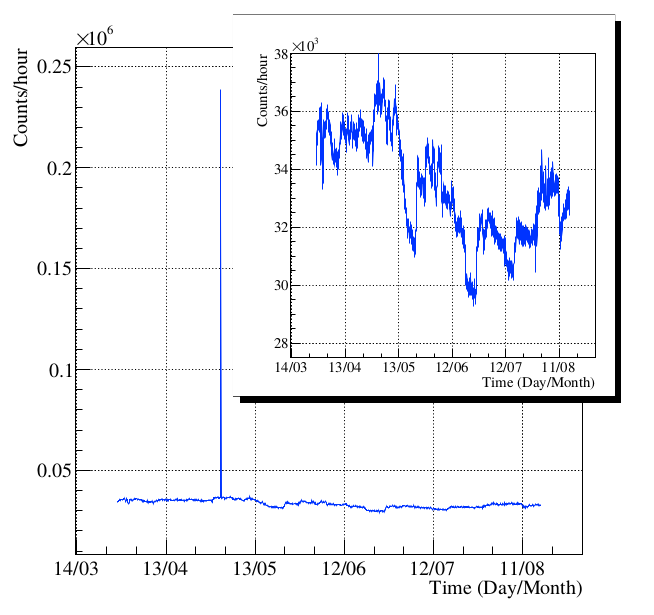
\includegraphics[scale=0.45]{7ExperimentalResultsDetectors/72ExperimentalResultsArrocampo/721TRITIUMAVEIRO0/BackgroundMeasurements.png}
\caption{Background measured with the TRITIUM-Aveiro prototype during its installation in Arrocampo dam \cite{ExperimentalPaperCarlos}.\label{fig:BackgroundArrocampoAveiro}}
\end{figure}
The data show good stability during the measuring period. An average rate of $9.31$ counts per second was obtained. A narrow peak is observed on May 2, 2019, caused by an opening of the roof of the lead shield to access the prototype. In the inset of the figure, the data are magnified for a better visualization. The MDA measured in Arrocampo dam for 60 minute integration time is 6 times larger than that obtained in the laboratory measurements, section \ref{subsec:TritiumAveiro}. This may be due to the electric noise introduced by the pumps of the water purification system and the inestability observed in the electronic boards.

The cosmic veto currently under development is planned to be installed and used in anti-coincidence along with two additional prototypes.

Furthermore, three TRITIUM-IFIC-2 prototypes and a cosmic veto, described above, are also planned to be installed in Arrocampo dam as soon as possible.